\chapter{Model}
\label{ch:Model}
\noindent

\section{Control flow in SpecTec prose}
\label{sec:spectecp}

% control flow structure in SpecTec prose
However, the \spectecp{} assumes a different model to explain the control flow
of WebAssembly.
Rather than using the notion of a pc, \spectecp{} assumes that WebAssembly
instructions are just given one by one.
This is because the \spectecp{} is generated automatically from the
\red{SpecTec DSL}.
\red{SpecTec DSL} uses rewrite rule to describe WebAssembly semantics, and it
is interpreted in \spectecp{} as consuming a WebAssembly instruction, pushing
or poping a control structures, and inputing new WebAssembly instructions.
It can be expressed in the following form:
$c^* \vdash i_0, i_1, ..., i_m \leadsto c'^* \vdash i'_0, ...i'_{m'}, i_1, ..., i_m$.
It means that given a sequence of contexts $c^*$, executing $i_0$ results in a
new sequence of contexts $c'^*$ and instructions $i'_0, ...i'_{m'}$.
To simply model the control flow of WebAssembly, other things not closely
related to the control flow are omitted in this notation.


% challenges in SpecTec prose
However, this viewpoint is challenged by the exiting label.
As the block structure doesn't remain intact in this model, it is hard to
describe \textbf{the end of the block}.
Furthermore, the exiting label is not performed by a specific WebAssembly
instruction, which makes it hard to model the behavior.
To handle this problem, an administrative instruction \texttt{end} is
introduced in \spectecp.
When entering a block, an \texttt{end} is appended to the end of the block.


% an example of Wasm control flow in official prose
\begin{figure}[h!]
    \centerline{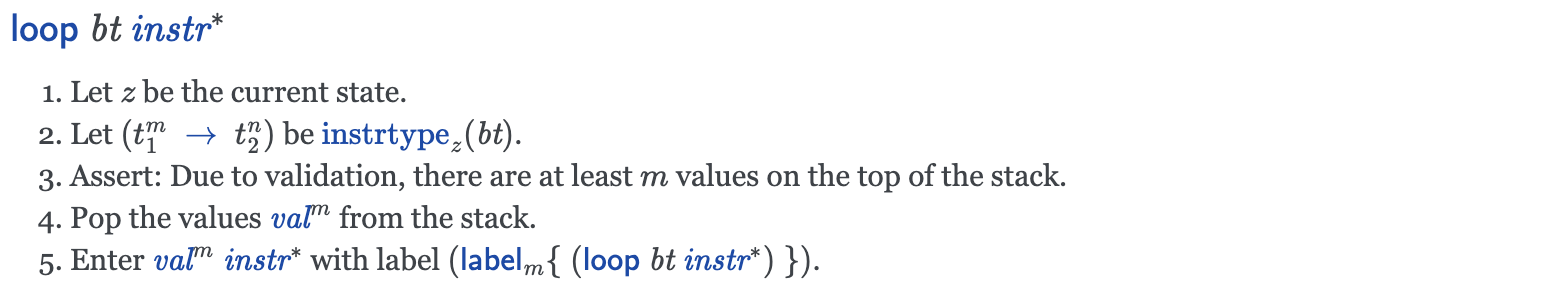
\includegraphics[width=15cm]{fig/spectec-loop}}
    \caption[Enter the caption title here]{SpecTec \texttt{loop}} \label{fig:spectec-loop}
\end{figure}
\begin{figure}[h!]
    \centerline{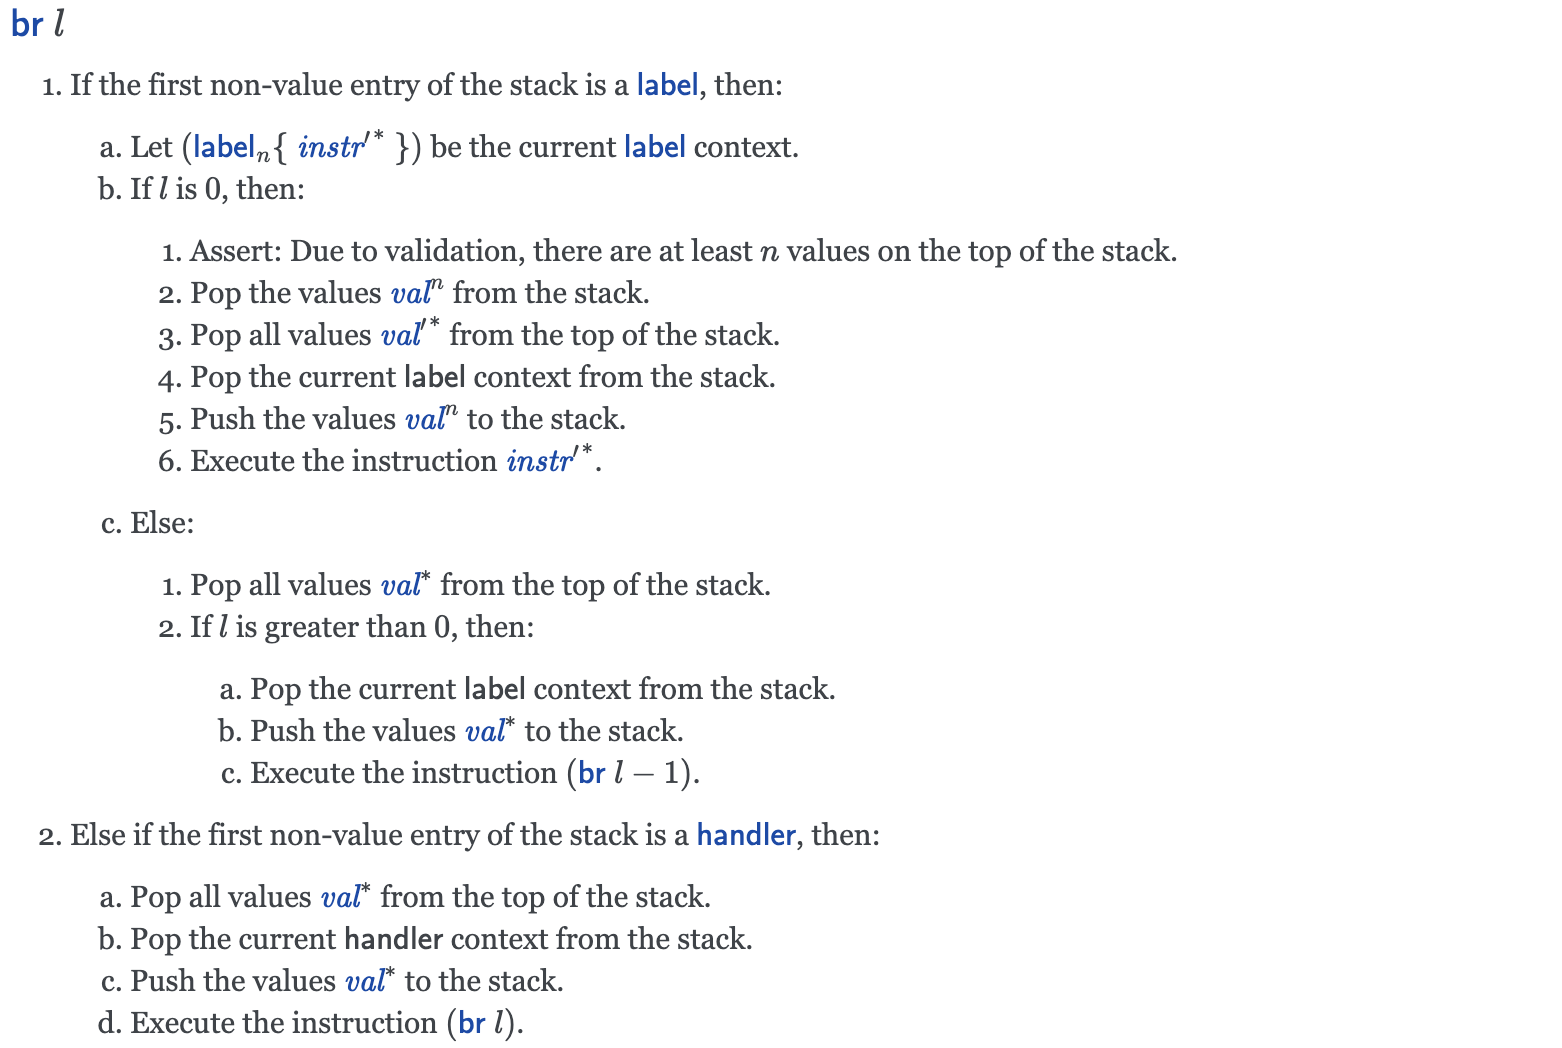
\includegraphics[width=15cm]{fig/spectec-br}}
    \caption[Enter the caption title here]{SpecTec \texttt{br}} \label{fig:spectec-br}
\end{figure}

\red{TODO: Change to array} \\
\begin{align}
  &c^*
  \vdash
  loop([ ~ i32.const ~ 42, ~ br ~ 0, ~ unreachable ~ ]), ~ unreachable
  \label{eq:loop-1} \\
&\leadsto
  label(loop([ ~ i32.const ~ 42; ~ br ~ 0; ~ unreachable ~ ])), c^*
  \vdash
  i32.const ~ 42, ~ br ~ 0, ~ unreachable, ~ end, ~ unreachable
  \label{eq:loop-2} \\
  &\leadsto
  label(loop([ ~ i32.const ~ 42; ~ br ~ 0; ~ unreachable ~ ])), c^*
  \vdash
  ~ br ~ 0, ~ unreachable, ~ end, ~ unreachable
  \label{eq:loop-3} \\
&\leadsto
  c^*
  \vdash
  loop([ ~ i32.const ~ 42; ~ br ~ 0; ~ unreachable ~ ]), unreachable
  \label{eq:loop-4}
\end{align}

Consider \cref{ex:br} above.
If we assume some control structure $c^*$ is given, the code can be expressed
like \cref{eq:loop-1}.
\cref{fig:spectec-loop} is the \spectecp{} of the \texttt{loop} instruction.
Rather than storing the point to jump as a continuation in the label, it stores
the \texttt{loop} instruction itself in the label, and \textit{enters} the
block.
Here, \textit{enter} means that it pushes the label in the stack and executes
the instructions in the block, which means that \texttt{i32.const},
\texttt{br}, \texttt{unreachable}, \texttt{end} and \texttt{unreachable} become
the new inputs in \cref{eq:loop-2}.
When \texttt{i32.const} is excuted, it pushes 42 as \officialp{} does
in \cref{eq:loop-3}.
The value is omitted for brevity.
However, \texttt{br} behaves a bit differently.
\cref{fig:spectec-br} is the \spectecp{} of the \texttt{br} instruction.
It pops the label from the stack, removes the input instructions until the end
of the block including the \texttt{end}, considers the loop instruction in the
label as a new input instruction.
Consequently, remaining inputs are \texttt{loop}, and \texttt{unreachable}
again in \cref{eq:loop-4}.
Therefore, it explains the same behavior in a different point of view.

\red{TODO: Also use example 3 to explain function call in official prose}

% an example of function call in official prose
\begin{example}
\label{ex:invoke}
\begin{verbatim}
  // function definition of $push42
  (func $push42 (result i32) (i32.const 42))

  // function call
  (call $push42) (f32.const 3.14)
\end{verbatim}
\end{example}

\red{TODO: Change to array} \\
\begin{align}
  &c^* \vdash call(\$push42), ~ f32.const ~ 3.14 \label{eq:call-1} \\
&\leadsto
  Label(\epsilon), ~ Frame, ~ c^* \vdash i32.const ~ 42, ~ end, ~ f32.const ~ 3.14 \label{eq:call-2} \\
&\leadsto
  Label(\epsilon), ~ Frame, ~ c^* \vdash end, ~ f32.const ~ 3.14 \label{eq:call-3} \\
&\leadsto
  c^* \vdash f32.const ~ 3.14 \label{eq:call-4} \\
&\leadsto
  c^* \vdash \epsilon \label{eq:call-5}
\end{align}

\cref{ex:invoke} contains a function definition whose body is \texttt{i32.const}, a
\texttt{call} instruction followed by a \texttt{f32.const} instruction, which
can be expressed in \cref{eq:call-1}.
By invoking a function, it pushes a frame and enters the block with a label in
\cref{eq:call-2}.
After executing the body in \cref{eq:call-3}, an \texttt{end} is executed.
In this point, this \texttt{end} represent both the end of the block and the
function.
As a consequence, this \text{end} perform both exiting label and returning from
a function in \cref{eq:call-4}, and the instruction after the \texttt{call} is
executed in \cref{eq:call-5}
It results in the values 42 and 3.14 pushed to the stack.


% summary & test
In short, the behavior of an \texttt{end} instruction 1) performs exiting
label, 2) looks up the top of the context, and 3) performs returing from a
function, if it is a frame.
The \spectecp{} can model the WebAssembly control flow using this \texttt{end}
instruction.
To show the correctness of the \spectecp{}, we run the WebAssembly tests
including official WebAssembly test suite by executing the \spectecp{} with
\red{definitional interpreter}.


% Problem
However, tests related to the control instruction are failed.
At that time, there was no explicit model to describe the control flow in
\spectecp{}, it was hard to define the problem, making it complicated to fix
the problem.



%%%%%%%%

% an example of buggy test case
\begin{example}
\label{ex:bug}
\begin{verbatim}
  // function definition of $br-returning
  (func  $brAndReturning (br 0) (unreachable))

  // function call
  (call $brAndReturning)
\end{verbatim}
\end{example}

\cref{ex:bug} contains a function that has only a \texttt{br} instruction, and a
\texttt{call} insstruction.
According to the \officialp{}, when the function \texttt{\$brAndReturning} is
called, a frame is pushed to the stack, and the block of the function
body is entered with a label.
When the \texttt{br} is executed, it pops the label from the stack.
As the end of the function is reached after the execution, returning from a
function is performed.
As a result, the frame is popped, so the call actually does nothing.


% explaination of the bug in SpecTec prose
\begin{align}
  &c^* \vdash call(\$brAndReturning) \label{eq:bug-1} \\
&\leadsto
  Label(\epsilon), ~ Frame, ~ c^* \vdash (br ~ 0) ~ (unreachable), ~ end \label{eq:bug-2} \\
&\leadsto
  Frame, ~ c^* \vdash \epsilon \label{eq:bug-3}
\end{align}

In \spectecp{} the call instruction in \cref{eq:bug-1} pushes a frame and
enters the function body \cref{eq:bug-2}.
When the \texttt{br} is executed, it pops the label and removes the input
instructions until the end in \cref{eq:bug-3}.
As a result, the frame is remained after the executing the call.
The problem is that the \texttt{br} should remove the end of the block but
should not remove the end of the function, but \texttt{end} express the end of
the block and the function at the same time.


% Fix
To fix the problem, semantics of \enteri is changed.
The sequence of contexts that is pushed in the AL algorithm is stored,
and when a block is entered, exiting label and returning from a function is
appended according to the sequence.


